\documentclass{article}

\usepackage{parskip}
\usepackage{graphicx}           % use \usepackage[demo]{graphicx} for all white pictures
\usepackage[section]{placeins}  % causes an implicit \FloatBarries to be used at the beginning of each section, so figure dont float into another section
\usepackage{wrapfig}            % lets text flow around a figure or a table: environments: wrapfigure, wraptable
\usepackage{float}              % does some beneficial stuff, dunno

\begin{document}
    Today it is about pictures.
    \begin{figure}[H]  % h: here, t: top, b: bottom, p: page, !: important
        \centering
        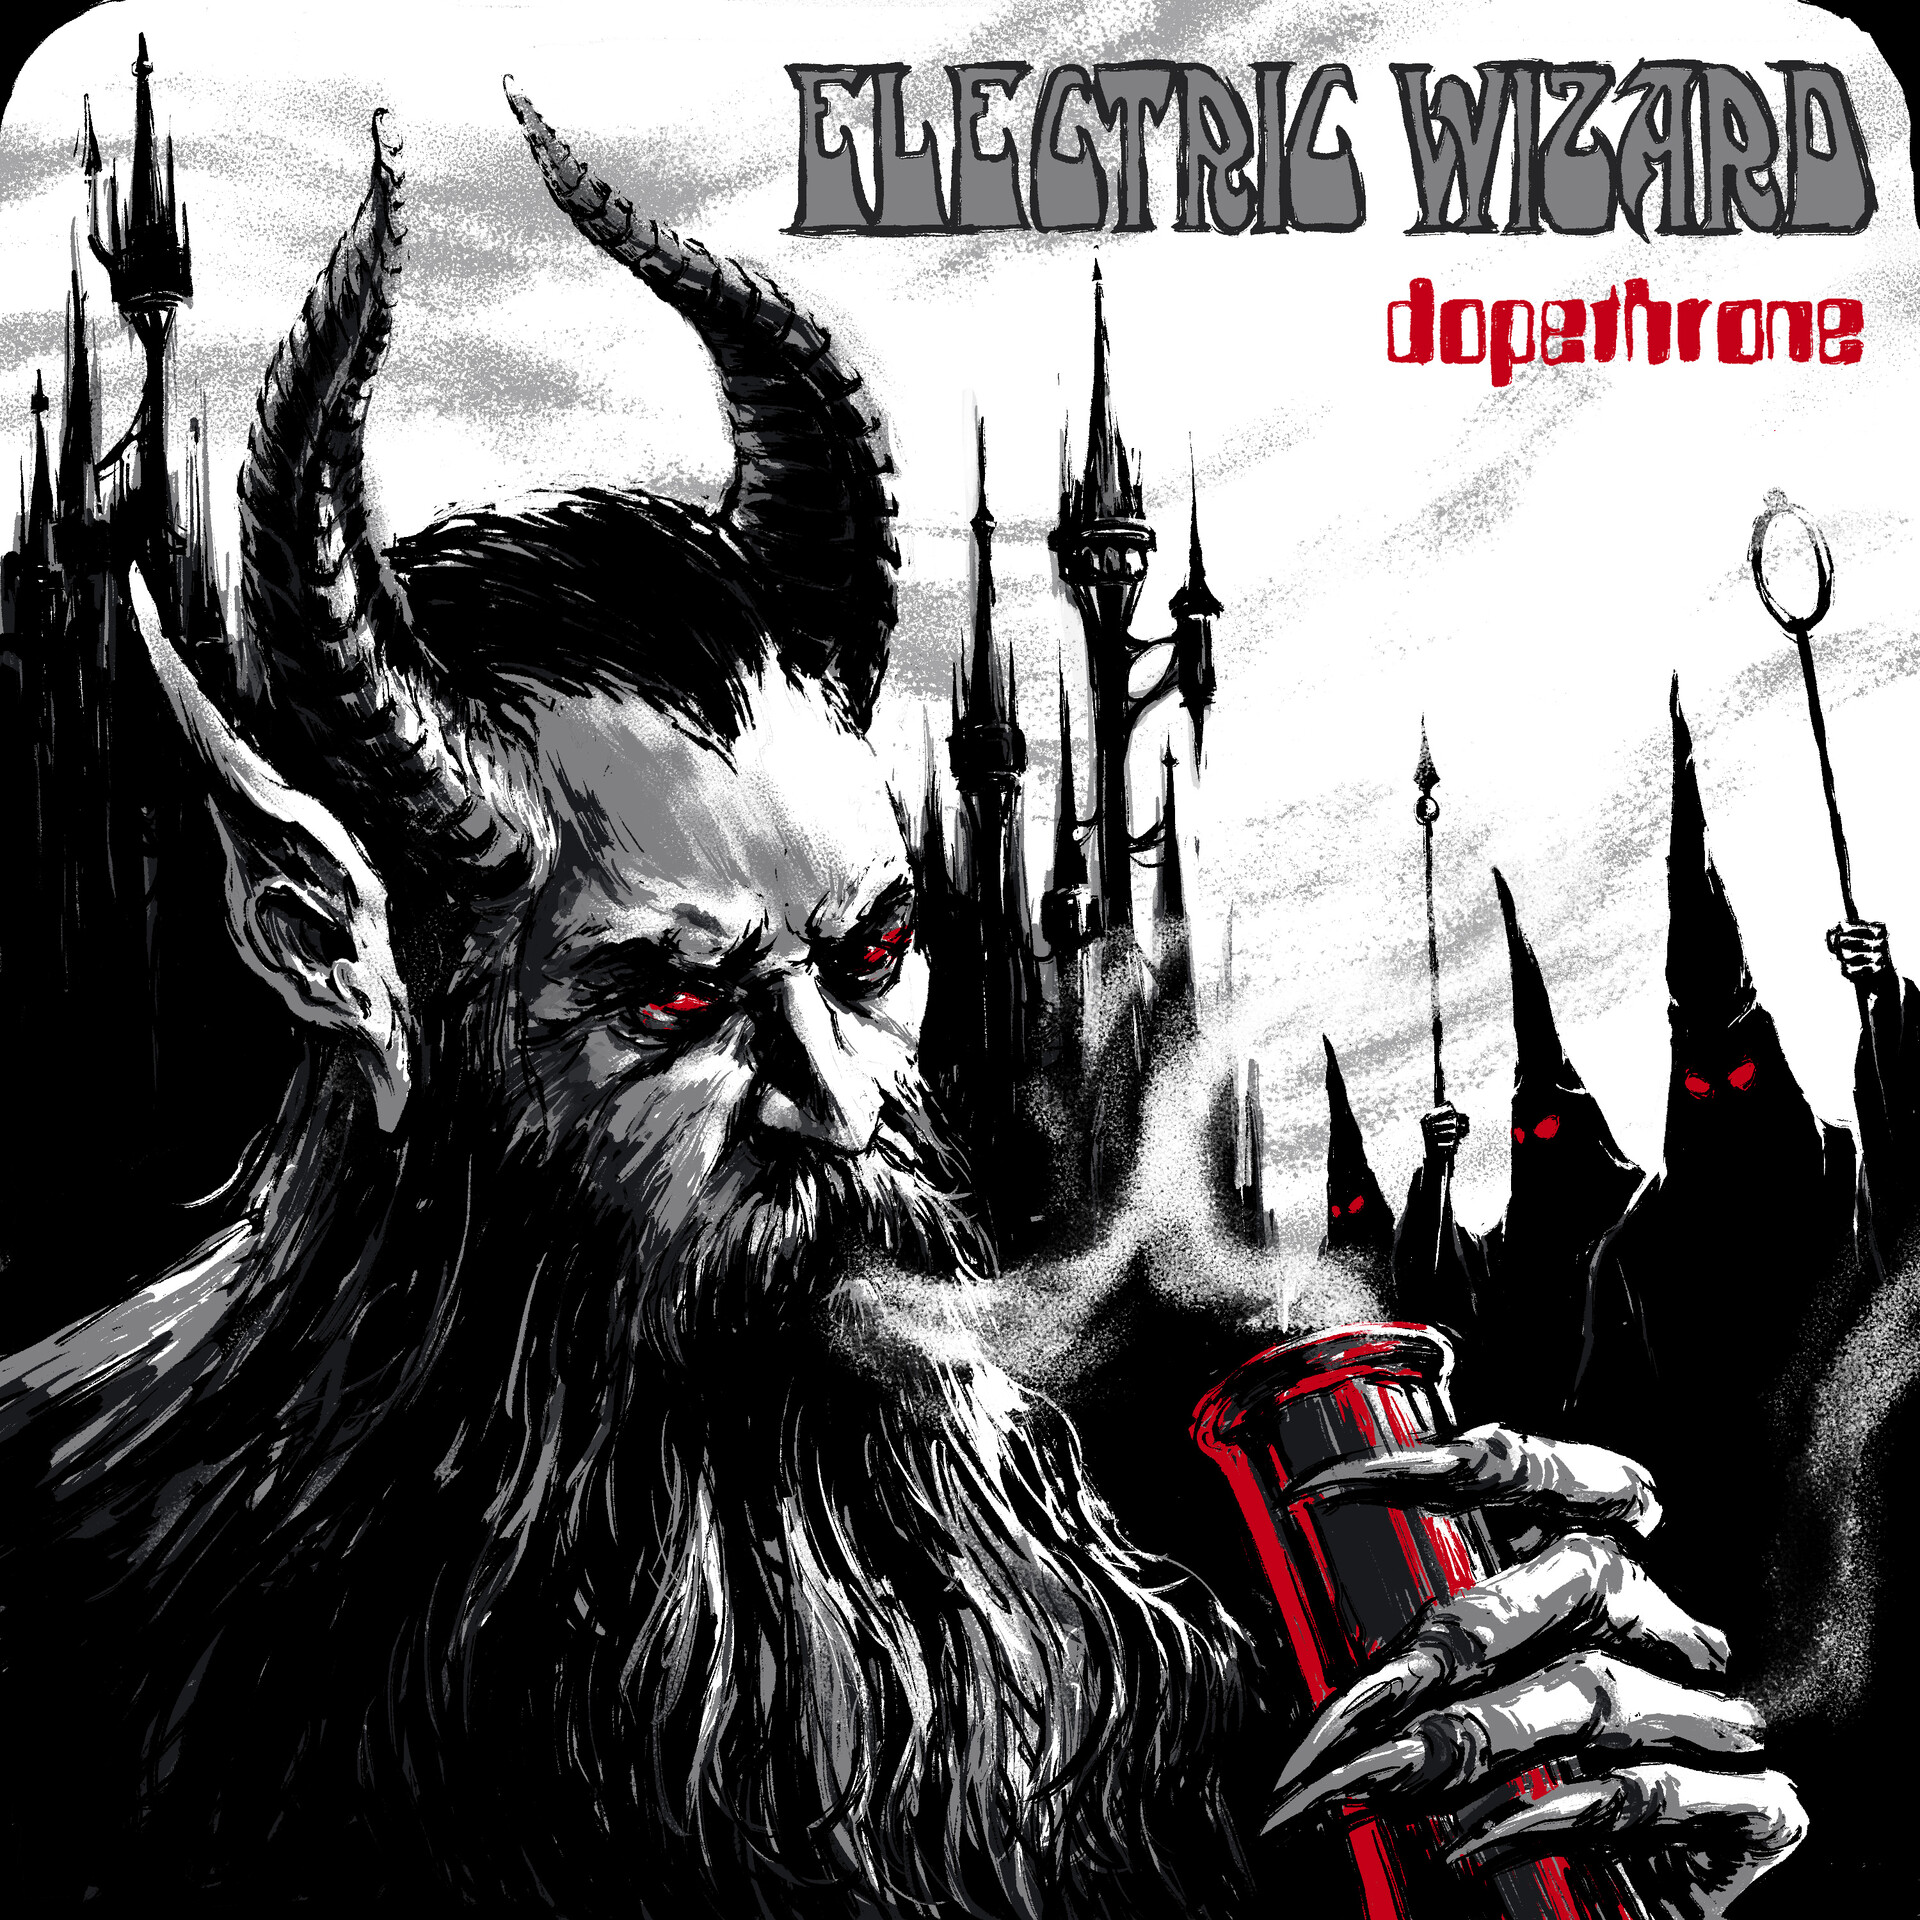
\includegraphics[scale=0.2]{./dopethrone.jpg} % arguments: width height scale angle
        \caption{Test figure}
    \end{figure}

    Another copy of previous image comes to rest.
    Other copy of previous image comes to rest.

    \begin{wrapfigure}{l}{5cm}          % rlio (inner, outer), RLIO for floating figure
        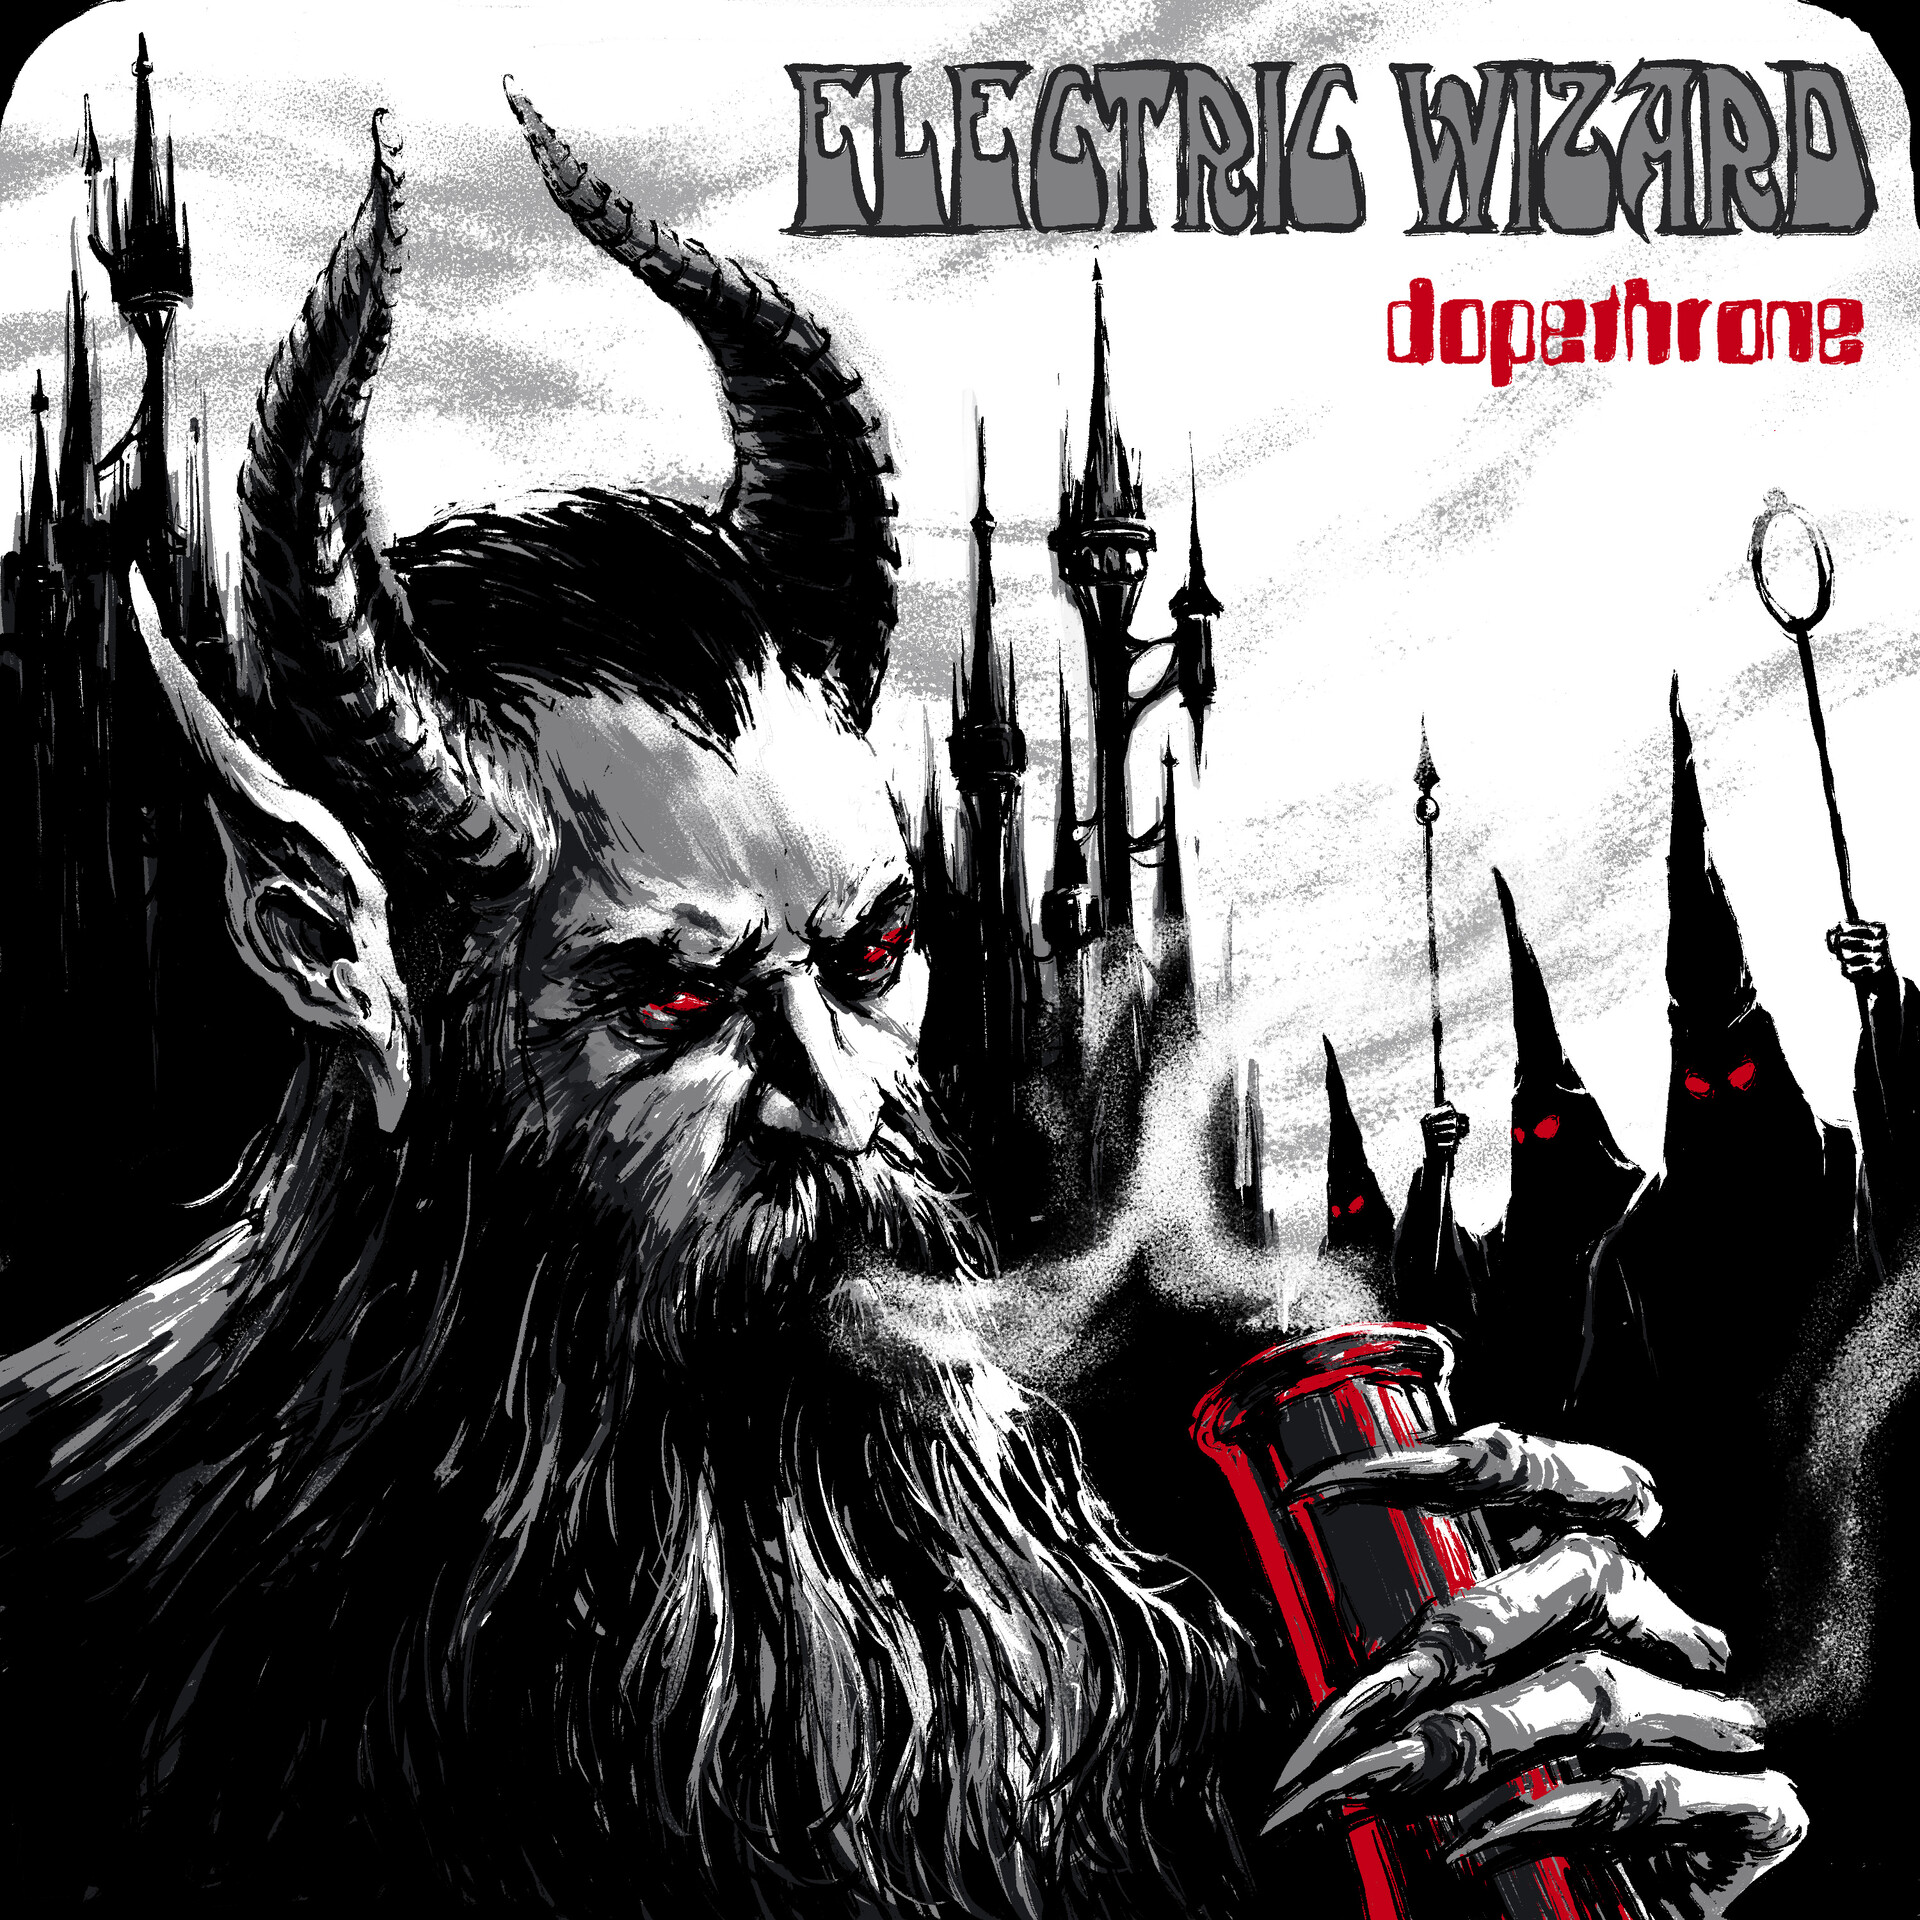
\includegraphics[width=5cm]{./dopethrone.jpg}
        \caption{Another one bites the dust.}
    \end{wrapfigure}
    Another copy of previous image comes to rest.
    Other copy of previous image comes to rest.
    Another copy of previous image comes to rest.
    Other copy of previous image comes to rest.
    Another copy of previous image comes to rest.
    Other copy of previous image comes to rest.
    Another copy of previous image comes to rest.
    Other copy of previous image comes to rest.
    Another copy of previous image comes to rest.
    Other copy of previous image comes to rest.
    Another copy of previous image comes to rest.
    Other copy of previous image comes to rest.
    Another copy of previous image comes to rest.
    Other copy of previous image comes to rest.
    Another copy of previous image comes to rest.
    Other copy of previous image comes to rest.
    Another copy of previous image comes to rest.
    Other copy of previous image comes to rest.
    Another copy of previous image comes to rest.

\end{document}
